\section{Results}

\subsection{\textit{mgrid} convergence}

The \textit{mgrid} parameter was varied from 200 until 500 in steps of 10 in order to find a fitting parameter which has an energy deviation of \(\leq 0.005 \text{ units}\) to its next higher cutoff.
The final value chosen to relabel the complete set of frames (test set and train set) is 500.

\begin{figure}
    \caption{Evaluation of the \textit{mgrid} cutoff parameter for DFT settings for the PBE functional in CP2K calculation.}
    \centering
    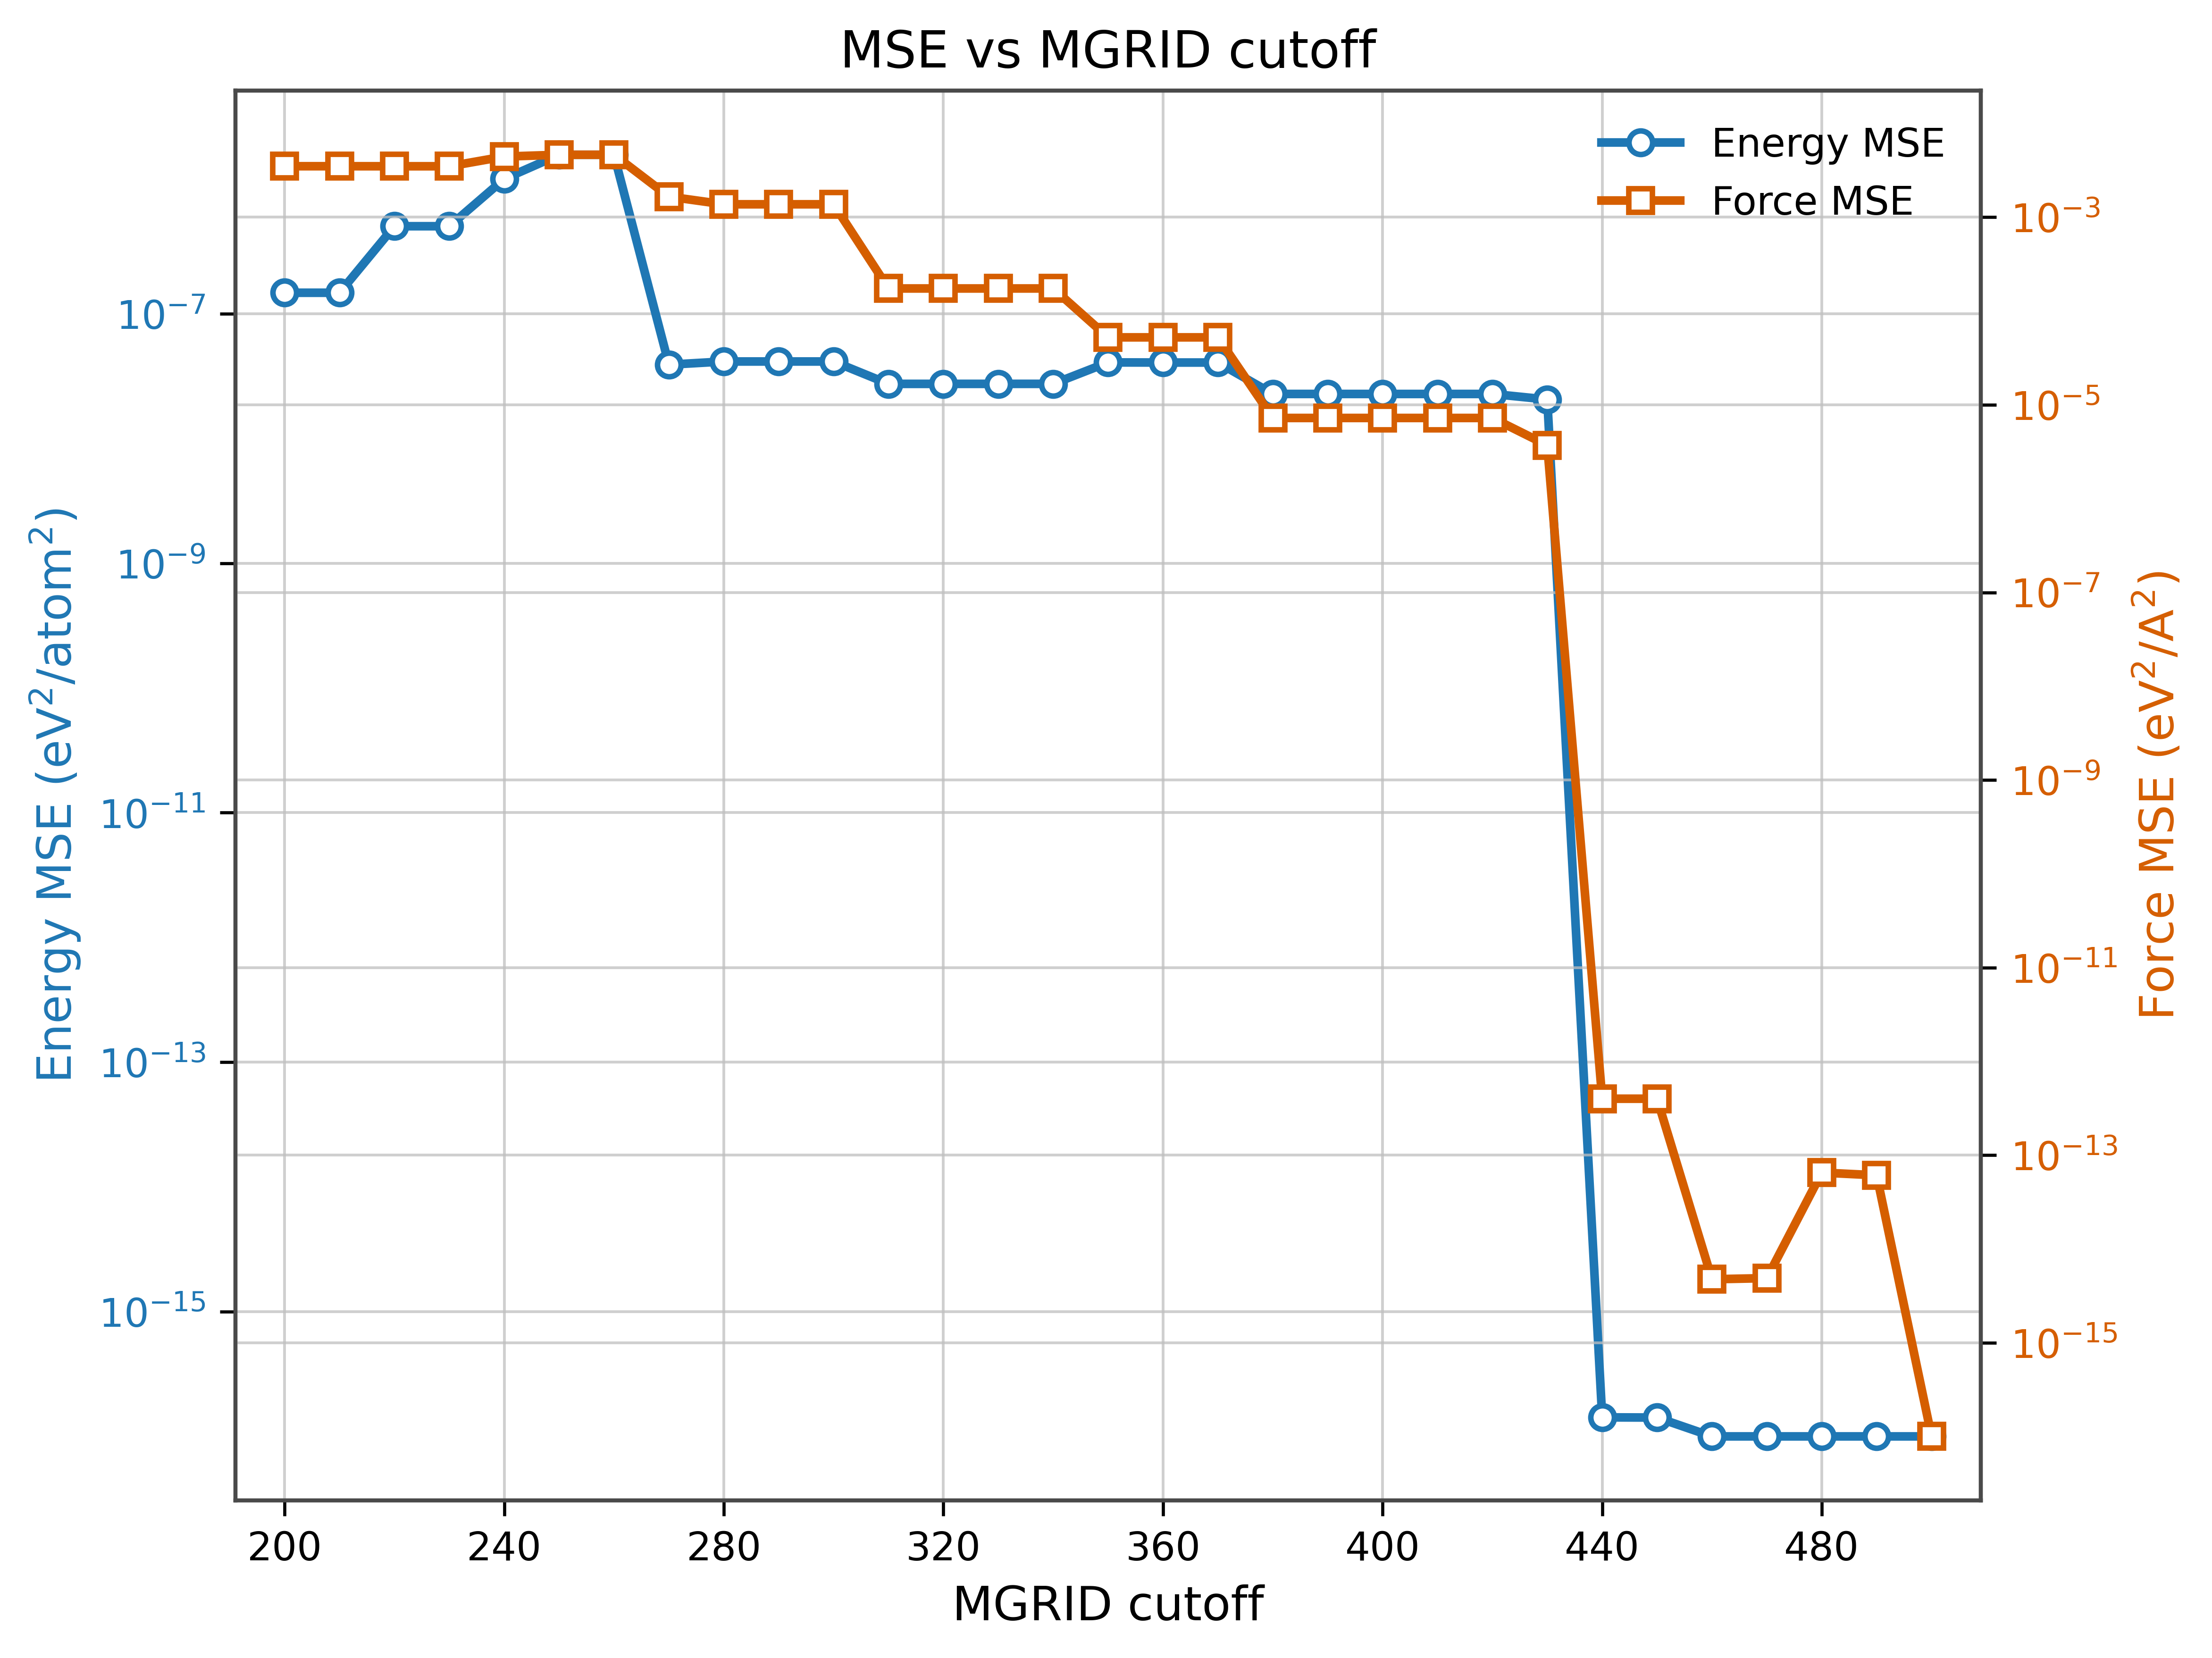
\includegraphics[width=.7\linewidth]{../mse_vs_mgrid.png}
    \label{fig:convergence}
\end{figure}

The convergence of the parameter over varying cutoff is shown in \cref{fig:convergence}.
In addition the Force MSE value can also be considered in the evaluation of the tradeoff for the \textit{mgrid} cutoff parameter, which in this case is also converged at 500.

\subsection{Hyperparameter Exploration}

As instructed on the worksheet, the influence of hyperparameters
\begin{enumerate}[label=(\Alph*)]
\item Radial Cutoff (\(r_{\text{max}}\)).
\item Network Architecture (number of hidden layers and their resprective number of neurons).
\item Number of Basis Functions (of the Neural Network).
\end{enumerate}
were investigated.

The baseline model which is represented in every subcathegory for comparison has the following parameters:
\begin{enumerate}
\item Radial Cutoff \(r_{\text{max}} = 5.5 \) \AA.
\item Network Architecture: Two hidden layers with each 32 neurons.
\item Number of Basis Functions: 24.
\item Maximal training epochs: 5000.
\end{enumerate}
Note that due to the convergence of a model during training, the patience evaluation of a training can end the training before reaching 5000 training epochs.

\paragraph{A: Radial Cutoff (\(r_{\text{max}}\)).}

\begin{figure}[htbp]
    \centering
    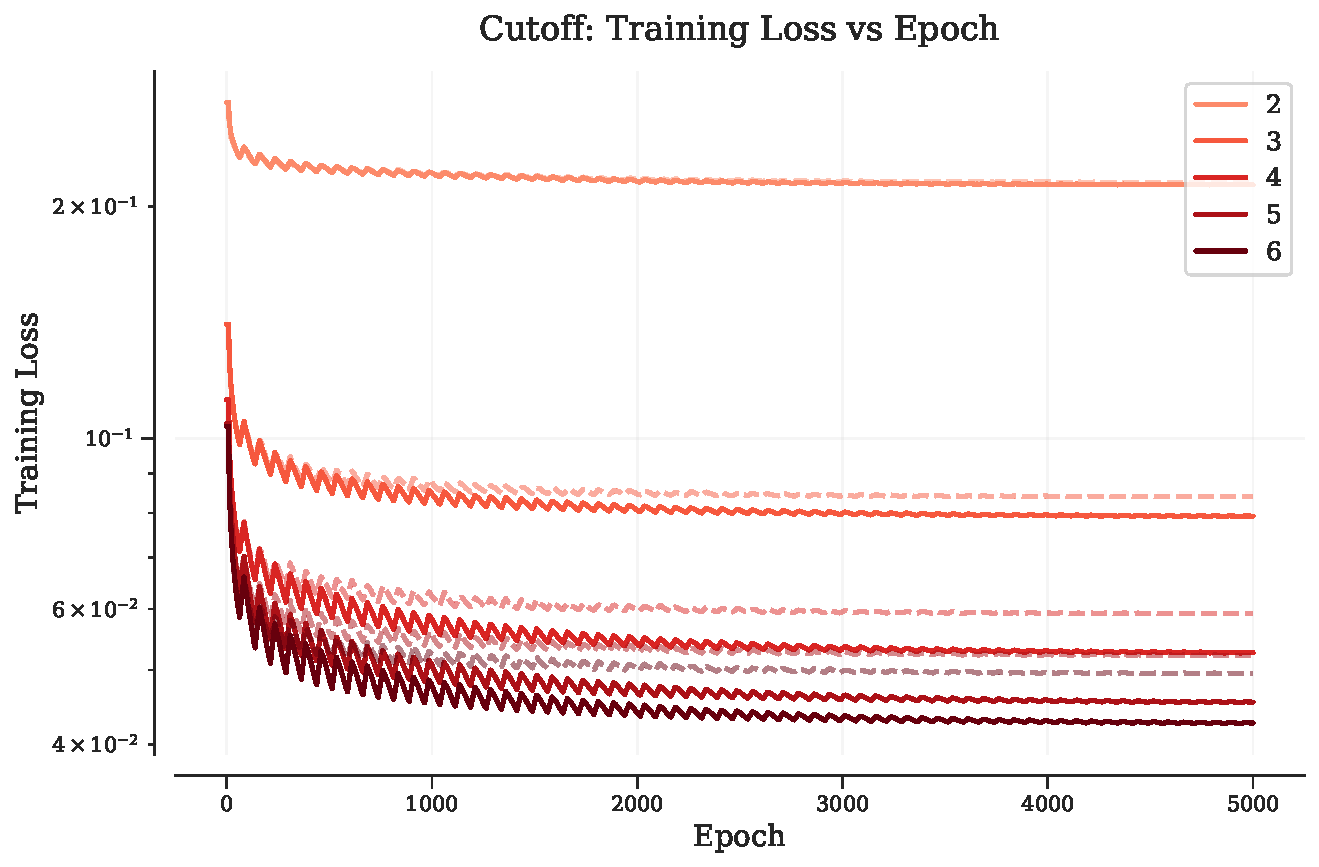
\includegraphics[width=.7\linewidth]{images/loss_cutoff.pdf}
    \caption{Evaluation of different Radial Cutoff (\(r_{\text{max}}\)) for the MLIP training.}
    \label{fig:cutoff}
\end{figure}

The results in \cref{fig:cutoff} show a reduction of the final training loss with increasing cutoff. Because the model training time did not increase significantly from increasing the cutoff, the highest value of 6 \AA is chosen to reach the highest accuracy.

\paragraph{B: Network Architecture.}

\begin{figure}[htbp]
    \centering
    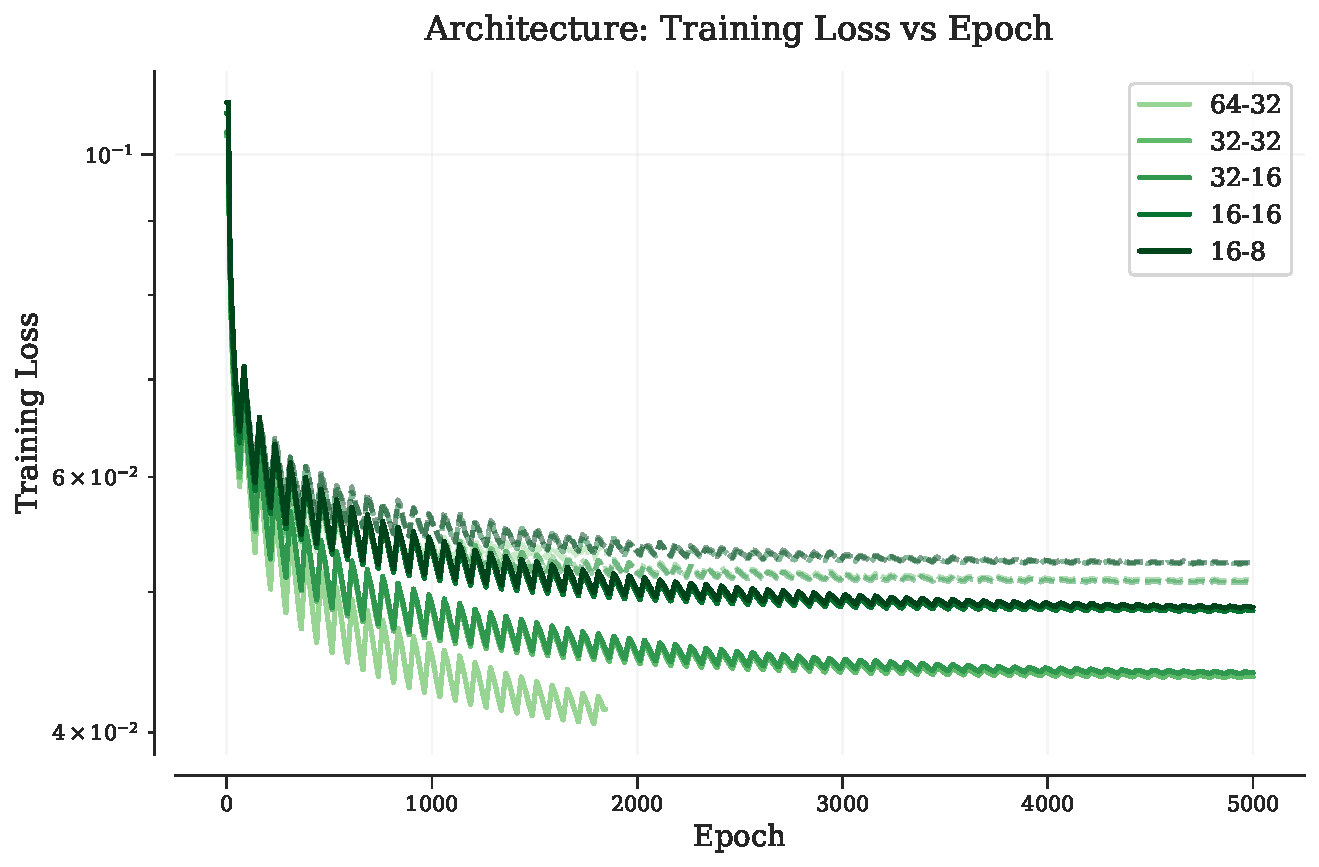
\includegraphics[width=.7\linewidth]{images/loss_architecture.pdf}
    \caption{Evaluation of different network architectures for the MLIP training.}
    \label{fig:architecture}
\end{figure}

The results in \cref{fig:architecture} show a reduction of the final training loss with increasing neuron size.
An interesting observation is that the first layer size seemingly has more influence on the final training loss than the second layer size.
Because of the early stopping of the \(64-32\) architecture, the final chosen architecture is \(32-32\).

\paragraph{C: Number of Basis Functions.}

\begin{figure}[htbp]
    \centering
    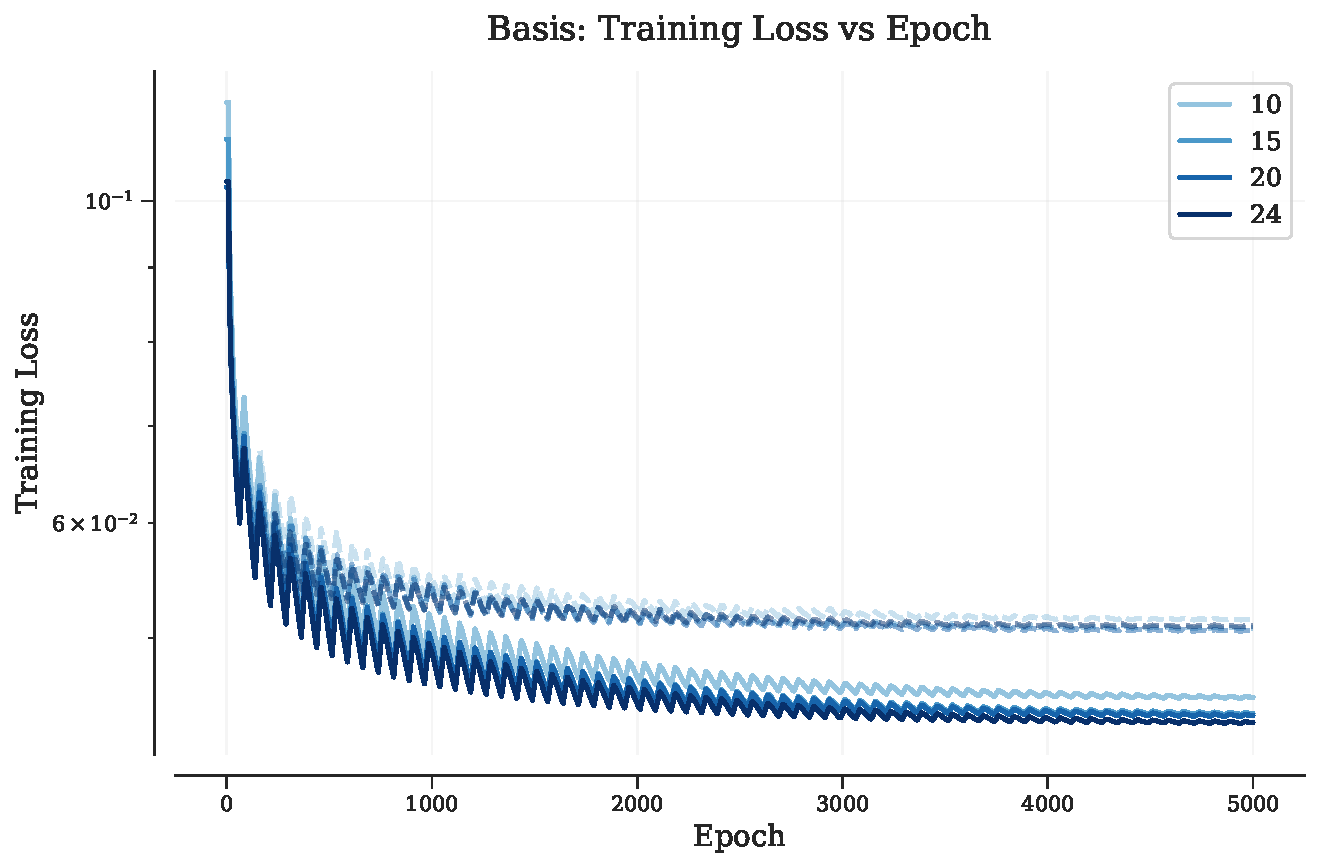
\includegraphics[width=.7\linewidth]{images/loss_basis.pdf}
    \caption{Evaluation of different numbers of basis functions for the MLIP training.}
    \label{fig:basis}
\end{figure}

The results in \cref{fig:basis} show a reduction of the final training loss with increasing number of basis functions.
The improvement of the final training loss seems to vanish for values over 20, but the increase of computational cost is minimal. That is why the final number of basis function is set to 24.

\paragraph{Comparison of every model}

\begin{figure}[htbp]
    \centering
    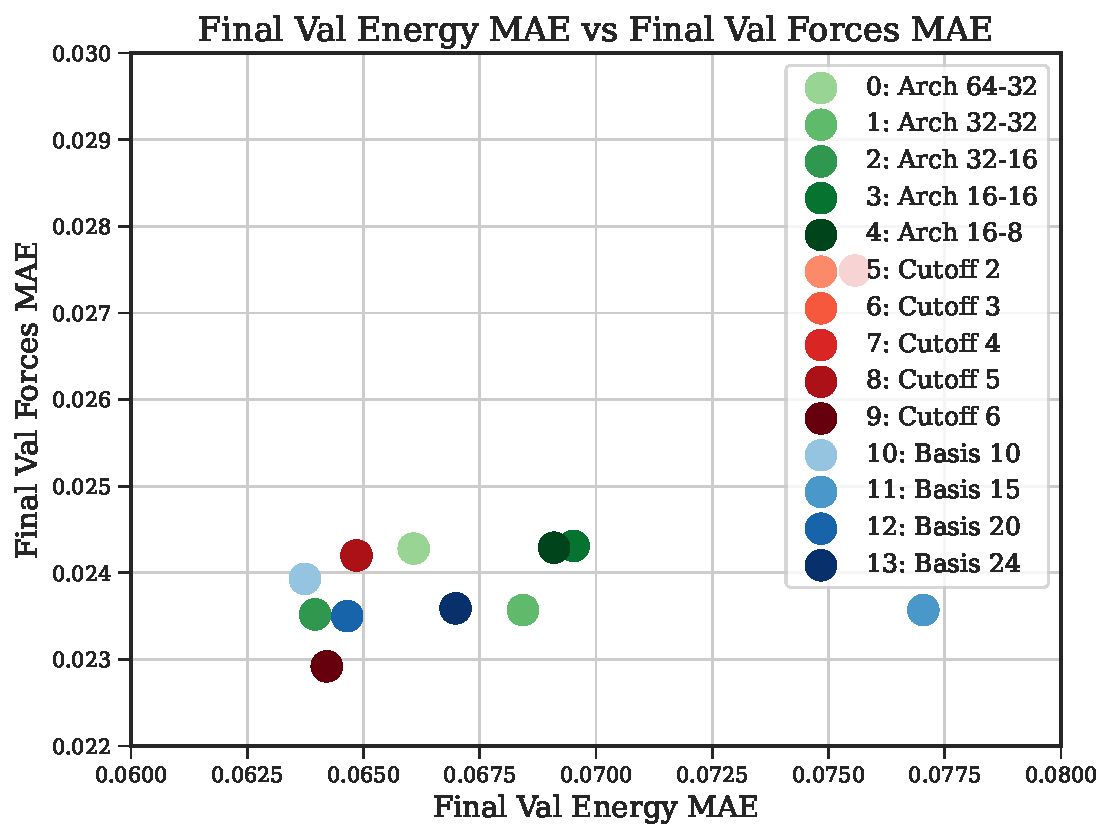
\includegraphics[width=.7\linewidth]{images/energy_force_mae.pdf}
    \caption{Evaluation of different neural network hyperparameter. The plot only compares the final force and energy MAE, not the final training loss.}
    \label{fig:comp_all}
\end{figure}

A complete comparison of the final loss for every model is shown in \cref{fig:comp_all}. This is only a comparison of the force and energy MAE at the end of every model training.

\subsection{Dynamical Analysis.}

After running a production simulation for 1 nanosecond with a box containing 64 molecules, we evaluate the self diffusion of the three different models (MACE, DFT, DFT+D3 correction).

\begin{figure}[htbp]
    \centering
    % Row 1
    \begin{minipage}{0.32\textwidth}
        \centering
        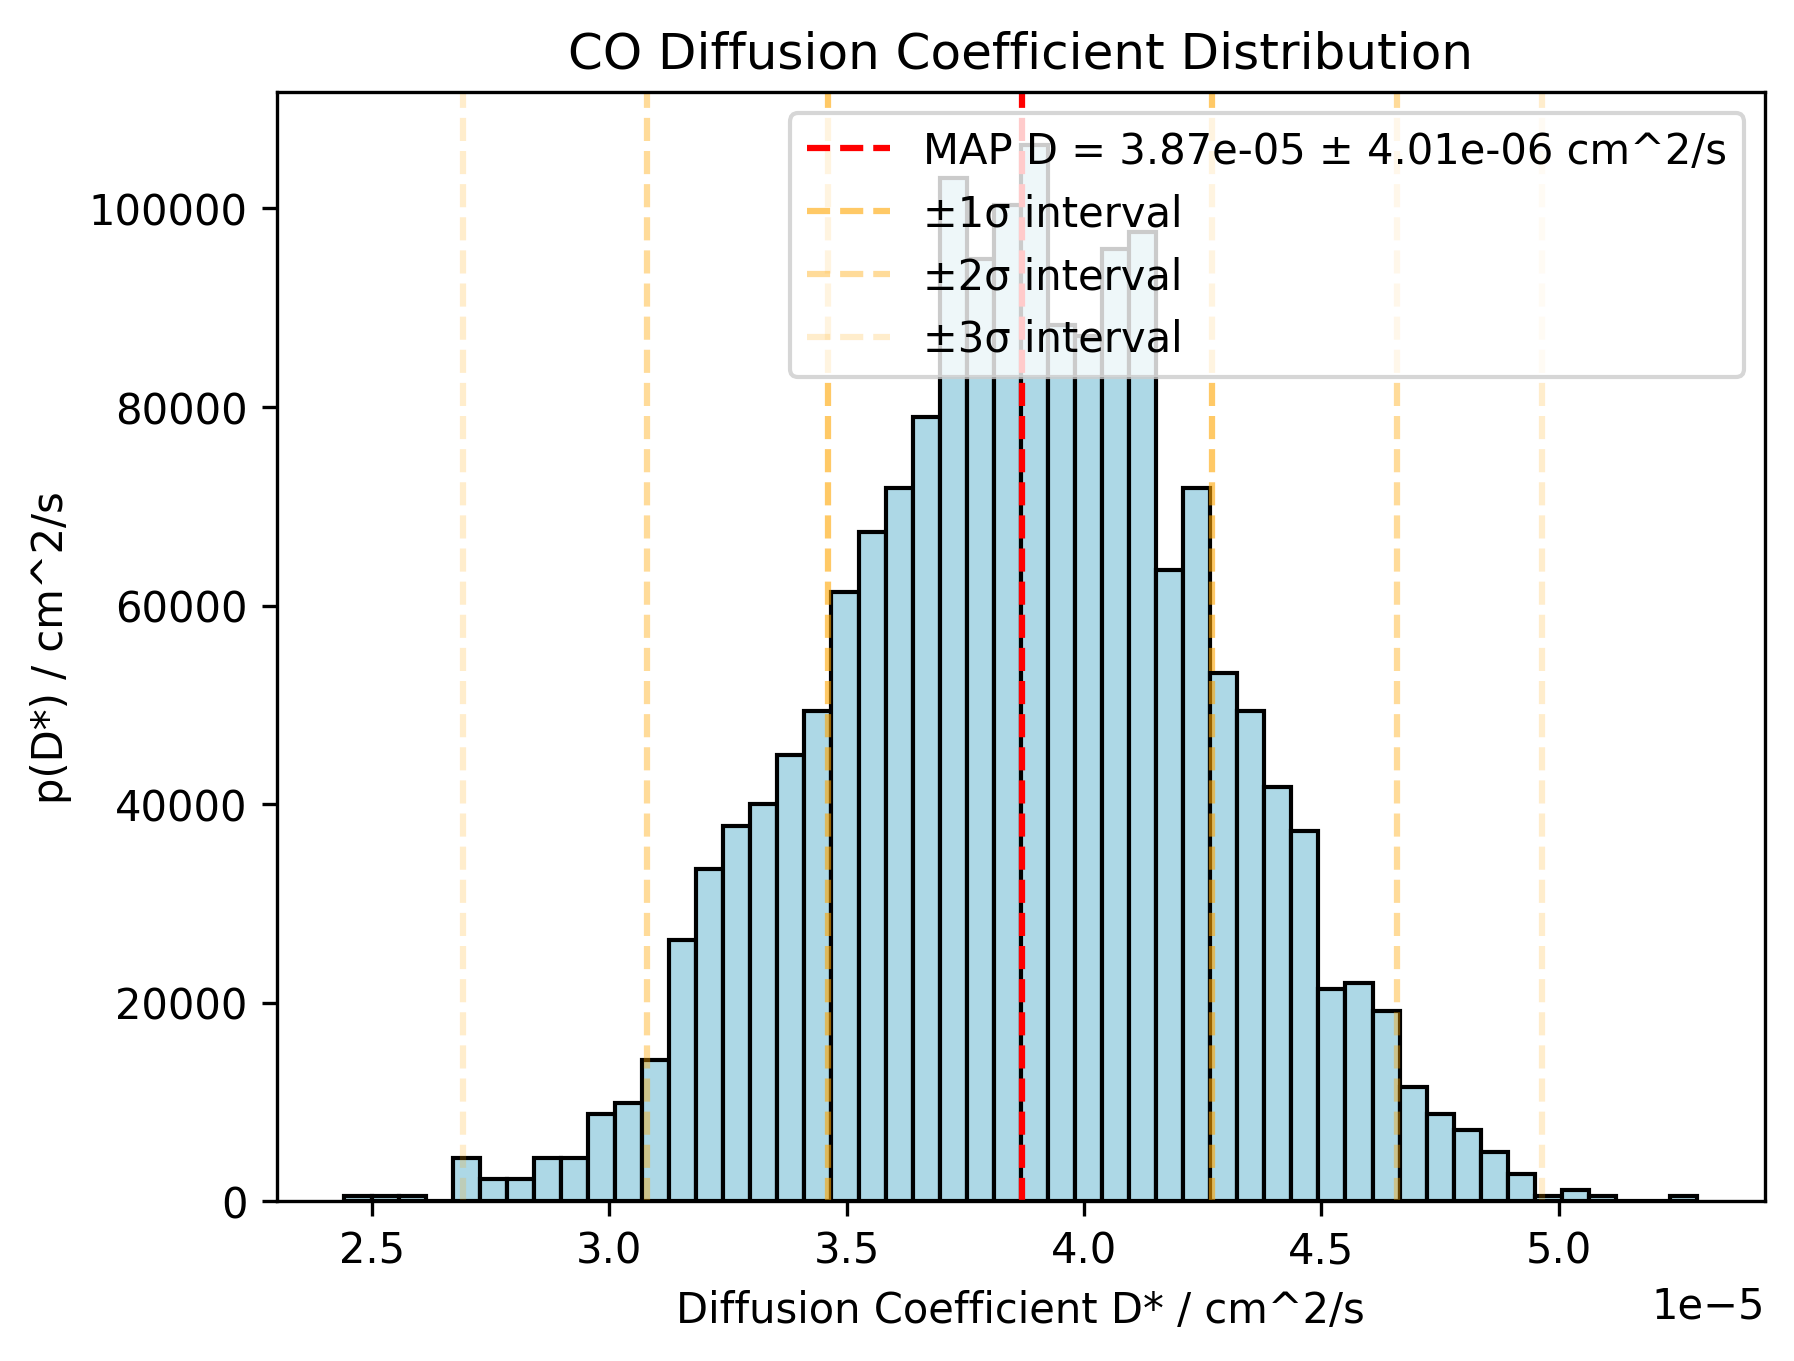
\includegraphics[width=\textwidth]{images/mace_hist.png}
        \subcaption{Histrogram: MACE Model}
    \end{minipage}
    \hfill
    \begin{minipage}{0.32\textwidth}
        \centering
        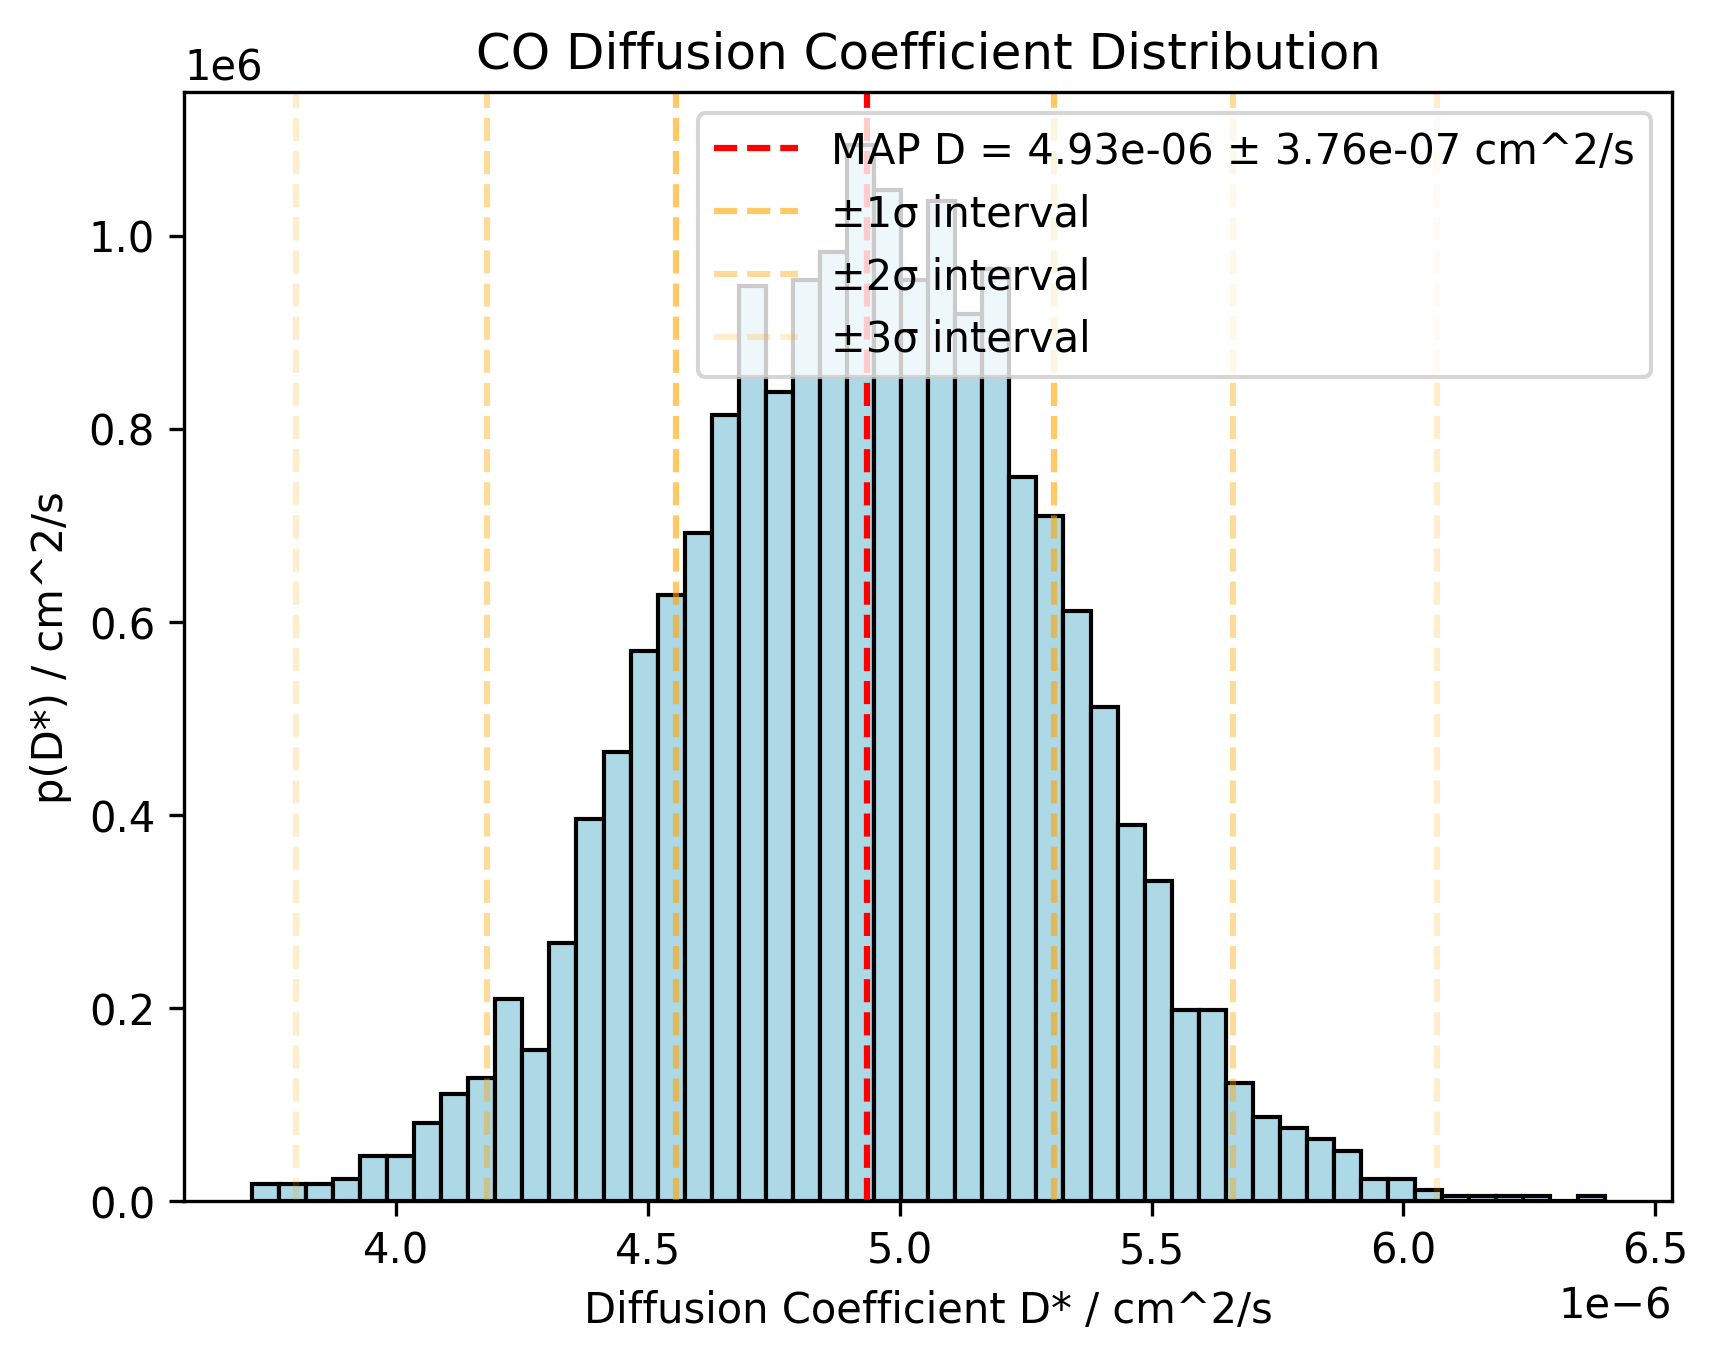
\includegraphics[width=\textwidth]{images/dft_hist.png}
        \subcaption{Histogram: DFT Model}
    \end{minipage}
    \hfill
    \begin{minipage}{0.32\textwidth}
        \centering
        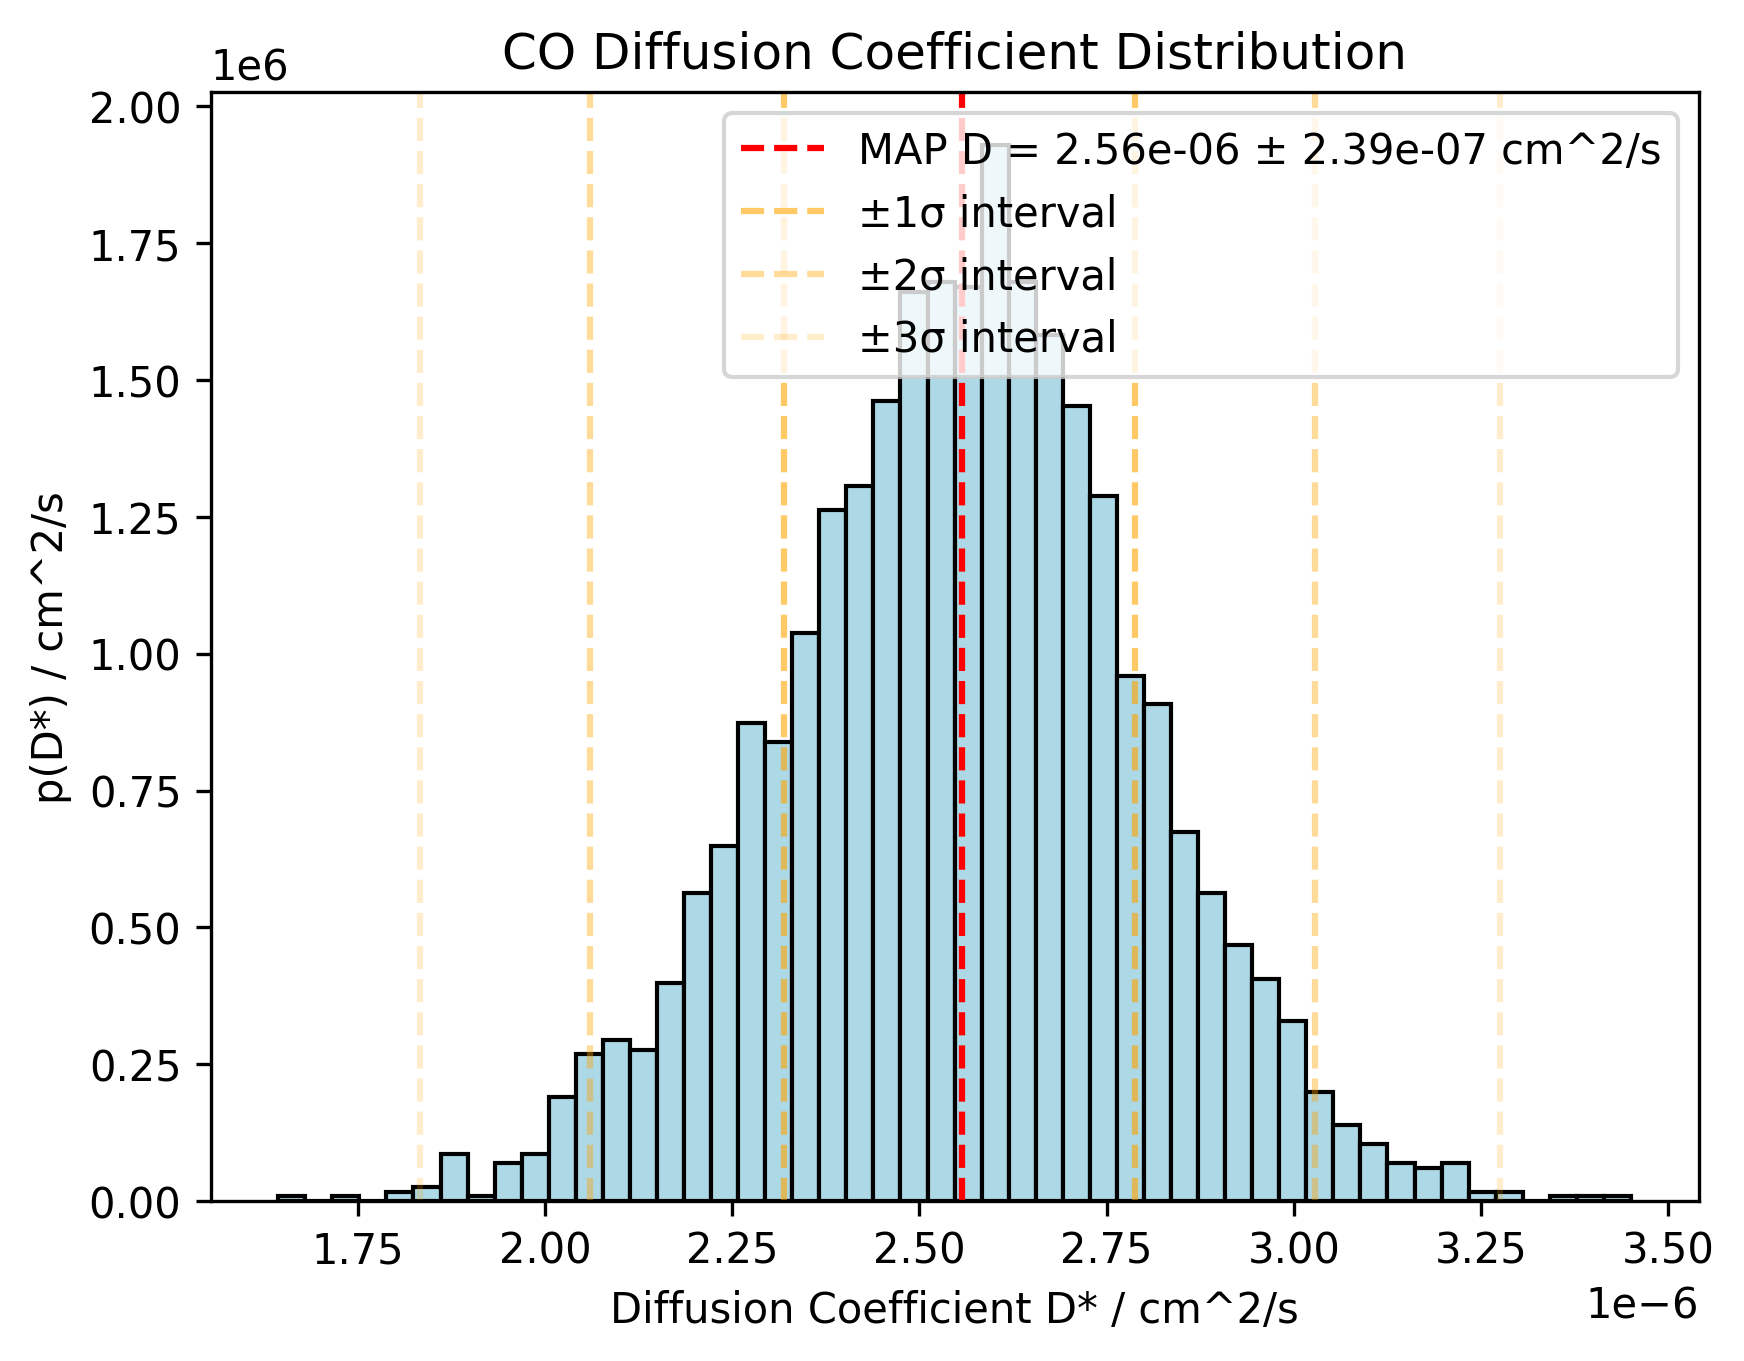
\includegraphics[width=\textwidth]{images/d3_hist.png}
        \subcaption{Histogram: DFT+D3 Model}
    \end{minipage}

    \vspace{0.5cm} % Vertical space between rows

    % Row 2
    \begin{minipage}{0.32\textwidth}
        \centering
        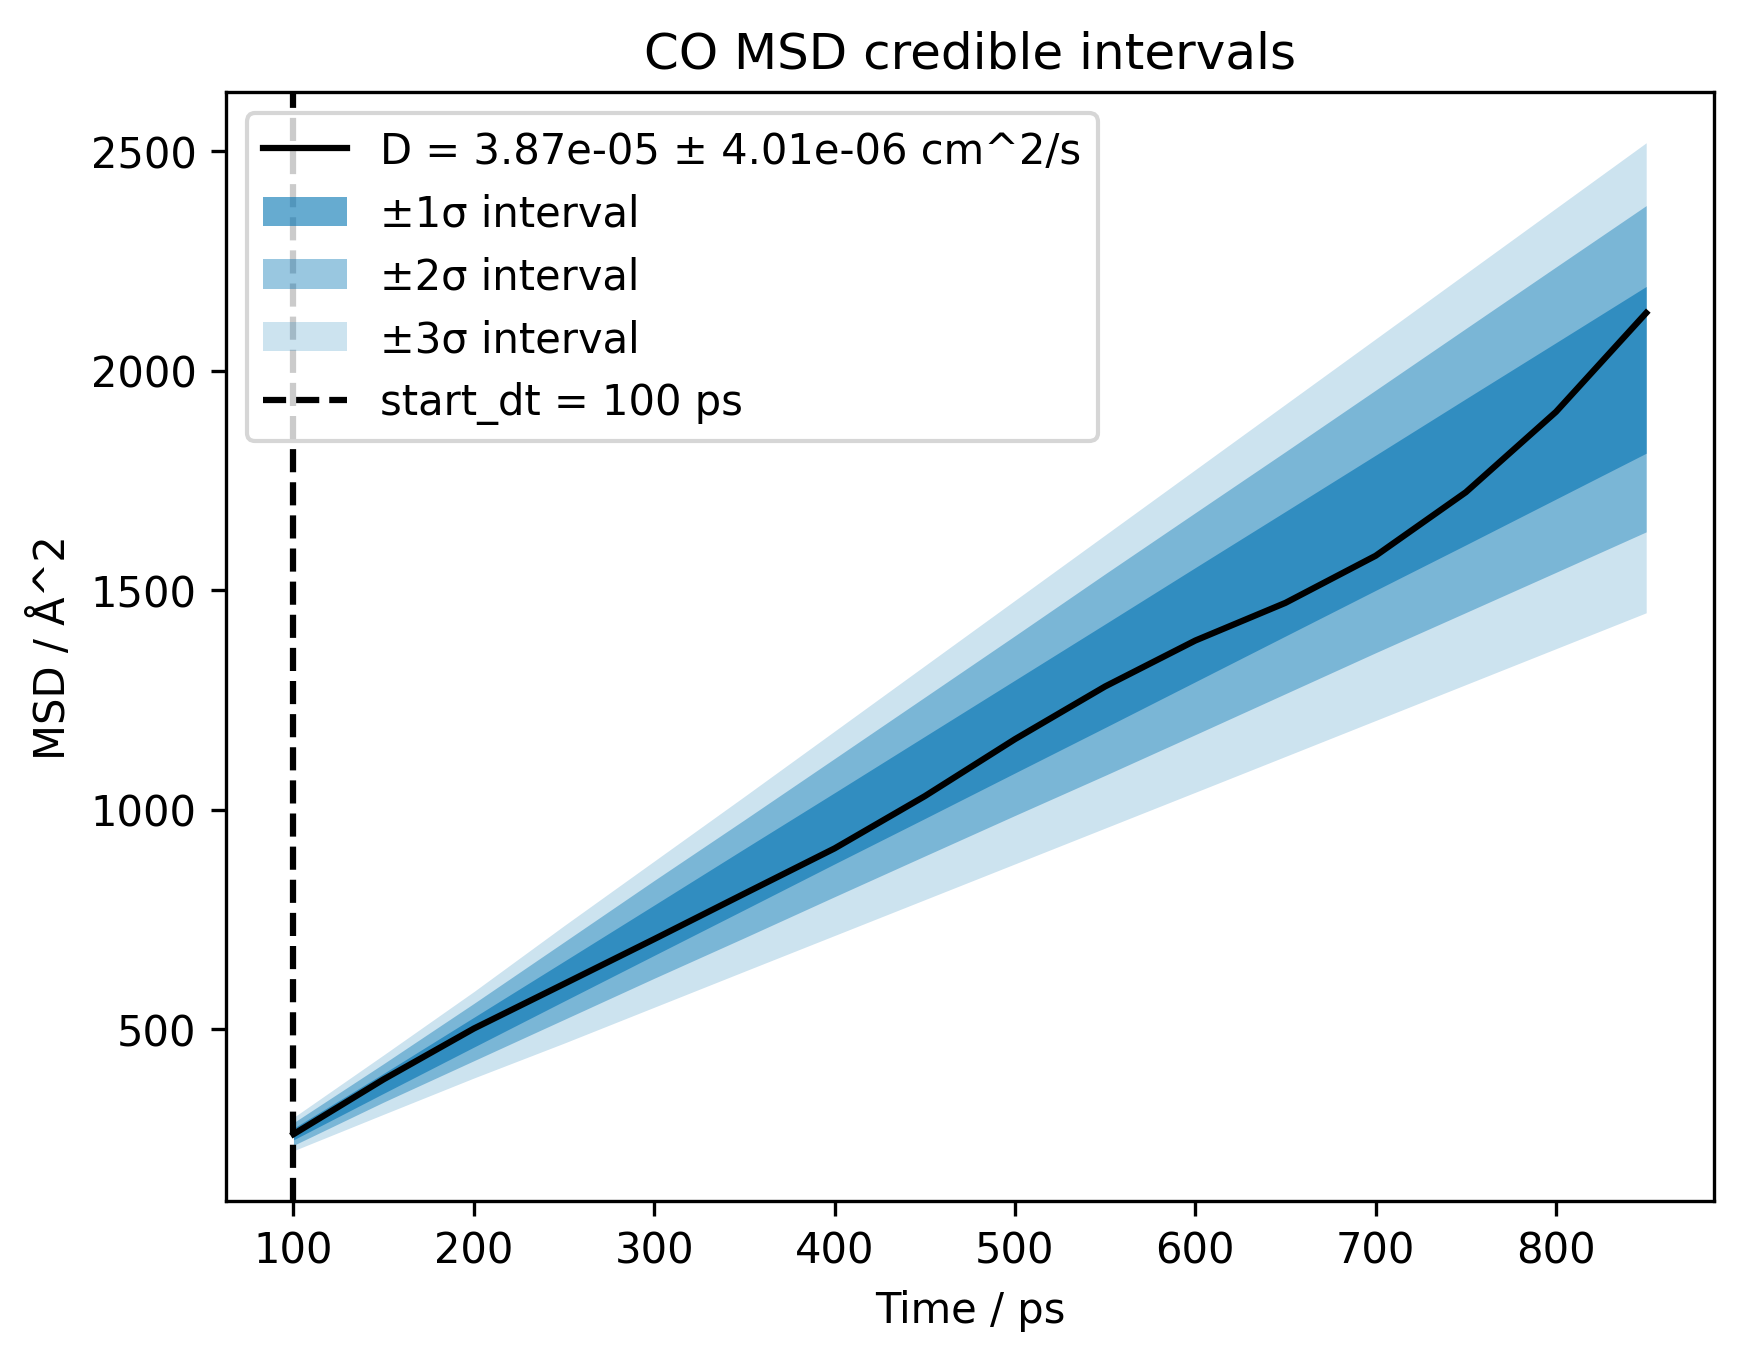
\includegraphics[width=\textwidth]{images/mace_msd.png}
        \subcaption{Bayesian Fit: MACE Model}
    \end{minipage}
    \hfill
    \begin{minipage}{0.32\textwidth}
        \centering
        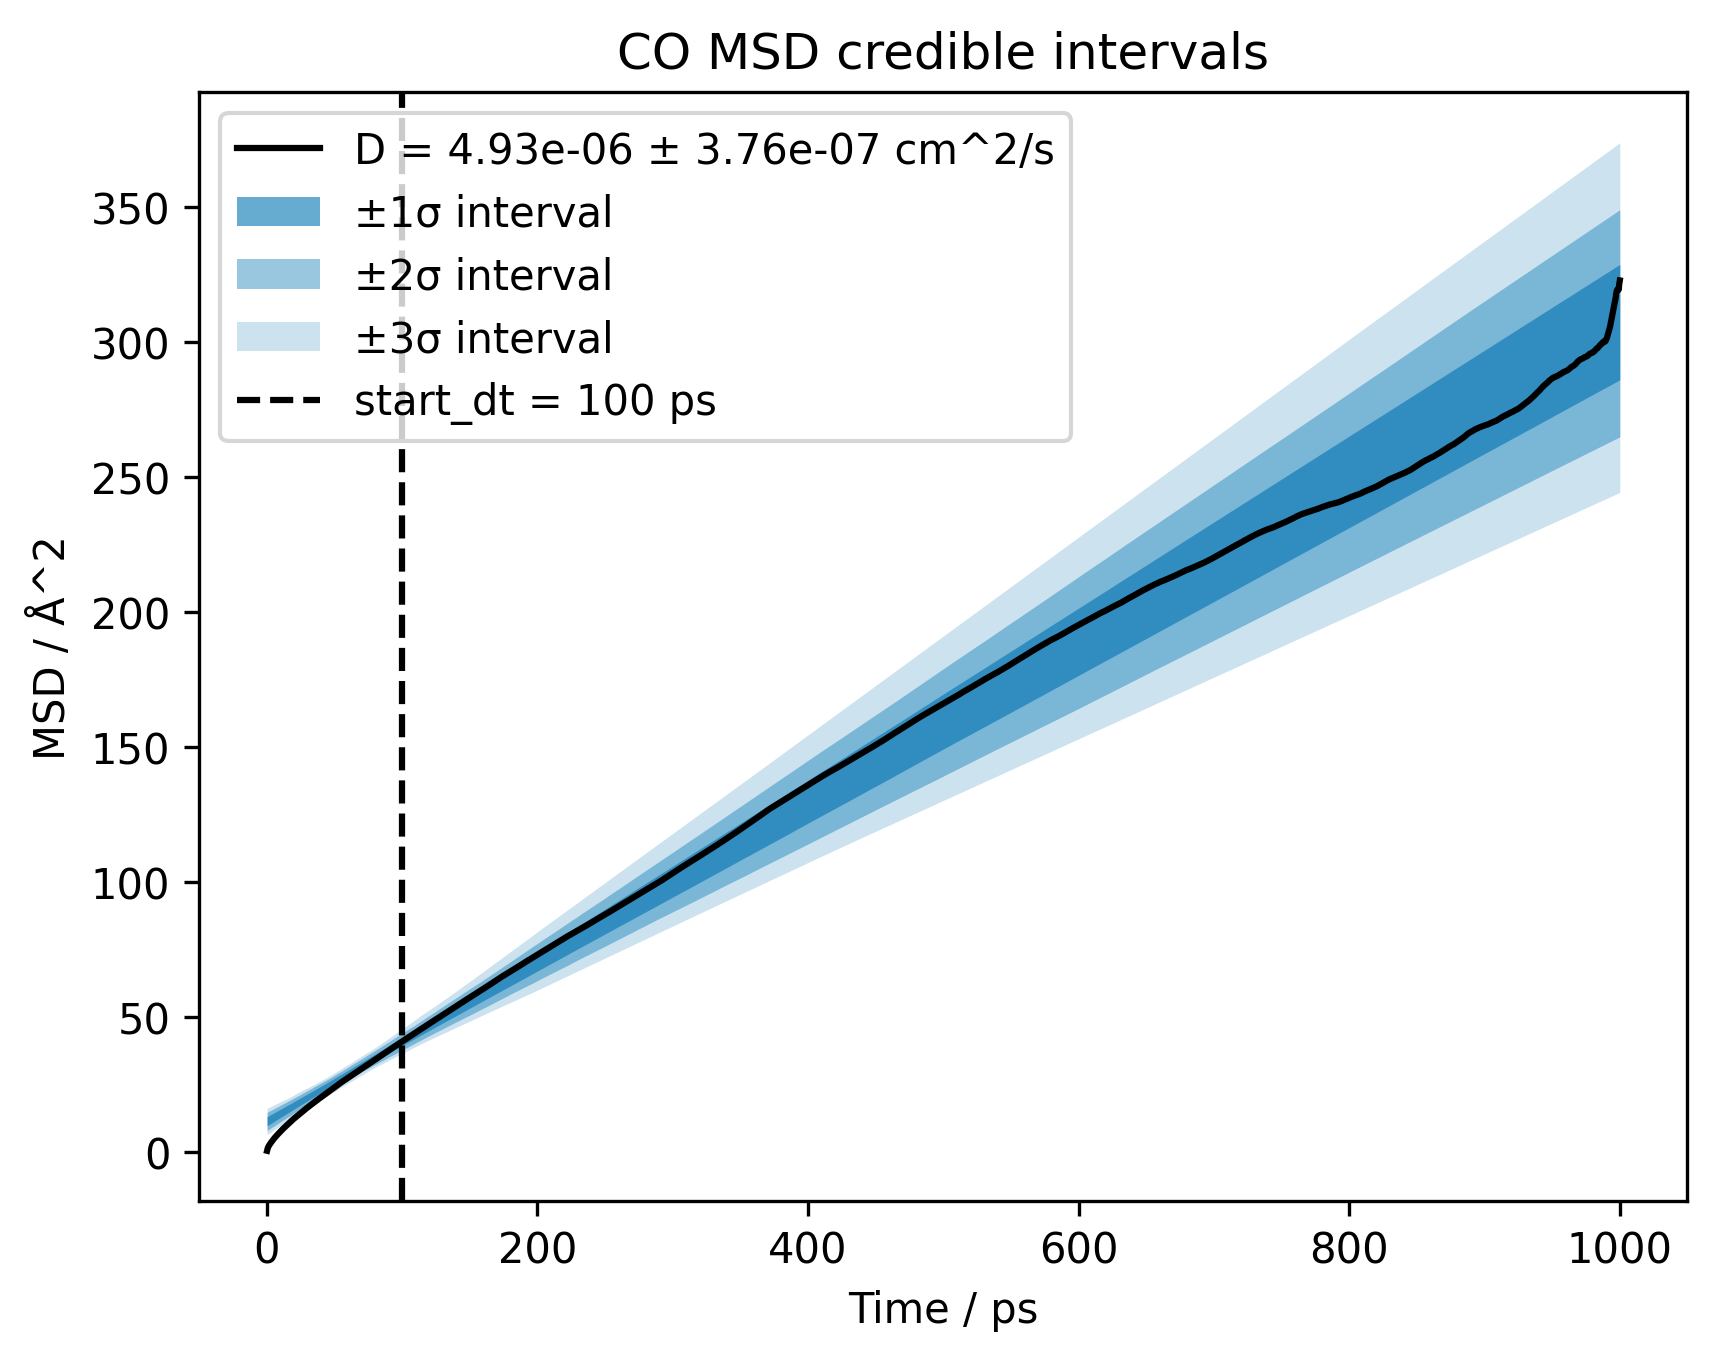
\includegraphics[width=\textwidth]{images/dft_msd.png}
        \subcaption{Bayesian Fit: DFT Model}
    \end{minipage}
    \hfill
    \begin{minipage}{0.32\textwidth}
        \centering
        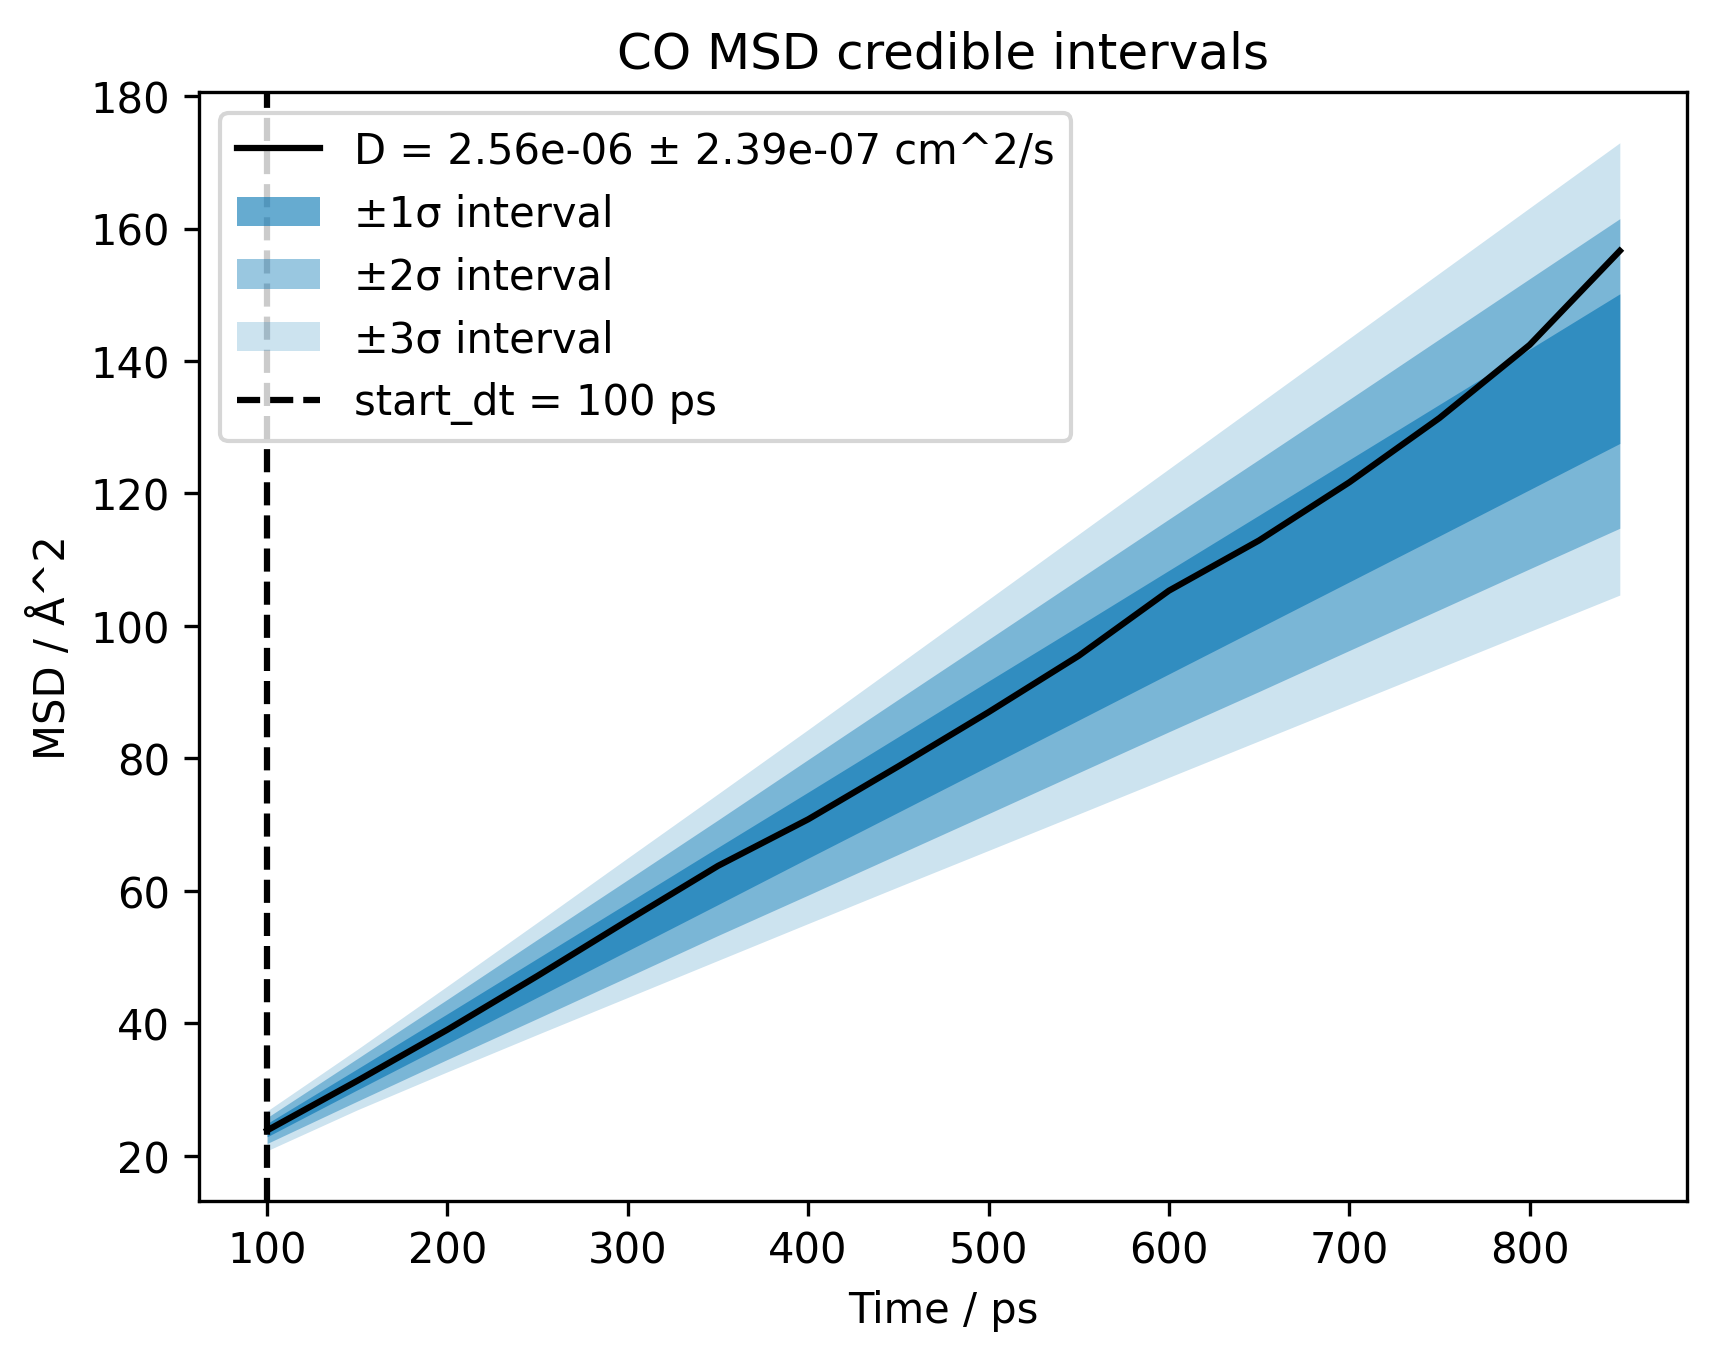
\includegraphics[width=\textwidth]{images/d3_msd.png}
        \subcaption{Bayesian Fit: DFT+D3 Model}
    \end{minipage}

    \caption{Evaluation of the self diffusion coefficient of the production MD simulations for three different models: MACE, PBE, PBE+D3 dispersion correction.}
    \label{fig:six_plots}
\end{figure}

The calculation of the diffusion coefficients done via Bayesian Fit and shown in \cref{fig:six_plots}.
The final values are

\begin{enumerate}[label=(\alph*)]
\item MACE: \(D \approx 2.5 \times 10^{-10} \, \text{m}^2/\text{s}\)
\item DFT: \(D \approx 5.2 \times 10^{-10} \, \text{m}^2/\text{s}\)
\item DFT+D3: \(D \approx 2.5 \times 10^{-10} \, \text{m}^2/\text{s}\)
\item Experimental value: \(D \approx 2.3 \times 10^{-10} \, \text{m}^2/\text{s}\) \cite{ijms23095011}.
\end{enumerate}

This means that in comparison to the "foundation model" MACE, the system specialized models, independend of the dispersion correction, already show a great improvement of the calculated diffusion coefficient, and therefore the diffusion behavior.

The dispersion corrected model seems to replicate the diffusion coefficient best, while the solely DFT based model overestimates the diffusion by approximately 100\%.

Further insight of the model performance is given via Radial Distribution Function comparison.

\subsection{Structual Analyis}

The most interesting bonds for structure analysis in methanol are the \(\text{O-H}\) bonds and the \(\text{O-O}\) bonds.
The \(\text{O-H}\) bonds show if the model can correctly replicate the tightest covalent bonds in the molecule while also giving insight to the nearest neighbor distance.

The \(\text{O-O}\) bonds are an even better measurement of the nearest neighbor distance and also allow for the calculation of the coordination number, quantifying the average number of neighbors in a "neighbor shell".

\paragraph{\(\text{O-H}\) Bonds}.

\begin{figure}[htbp]
    \centering
    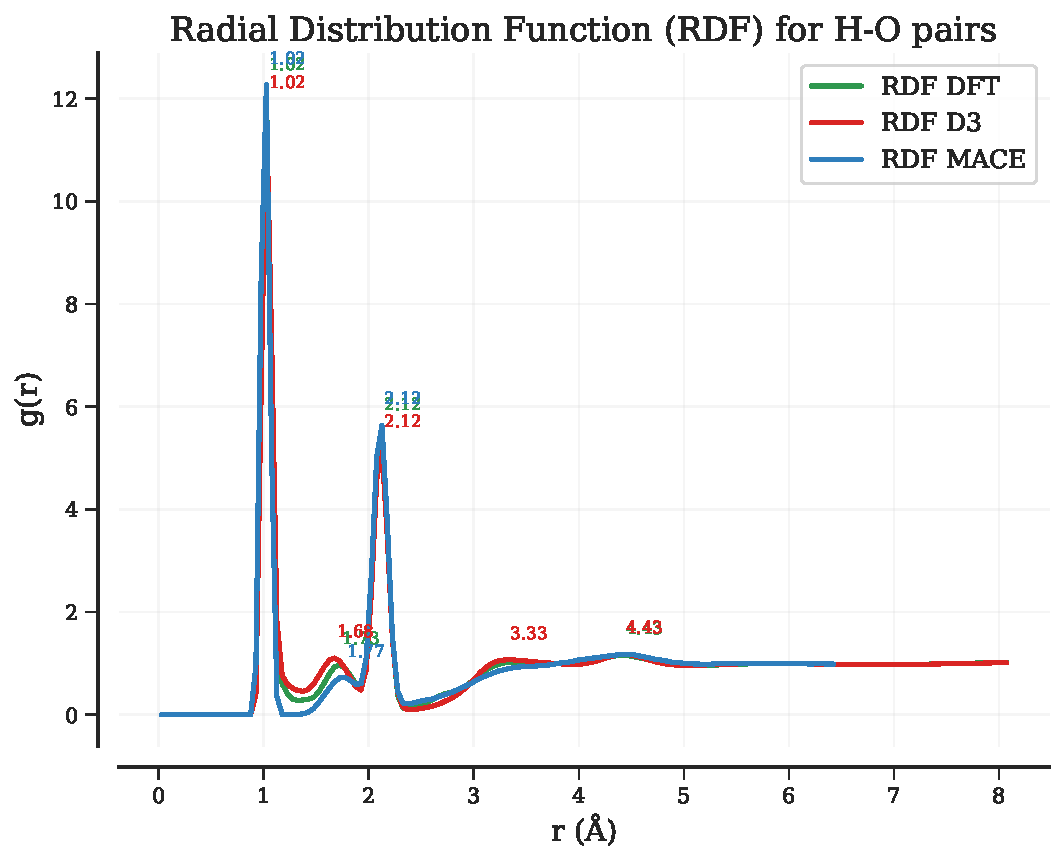
\includegraphics[width=.7\linewidth]{images/rdf_o_h.pdf}
    \caption{Radial distribution function of three models compared for the \(\text{O-H}\) bonds.}
    \label{fig:oo}
\end{figure}

Over all the models show a good agreement on the first peak of the RDF (\cref{fig:oo}). The first average hydrogen bond distance is \(r_1 \approx 1.02\)\AA. The experimental value is \(r_1 \approx 0.96\)\AA, showing that each model underestimates the hydrogen bond strength.
Same observation can be made for the nearest neighbor distance \(r_2 \approx 2.12\)\AA. The experimental value is \(r_2 \approx 2.08\)\AA, also hinting a slight underestimation of intermolecular attaction.
An important observation is, that no overstructuring due to dispersion correction is visible.


\paragraph{\(\text{O-O}\) Bonds}.

\begin{figure}[htbp]
    \centering
    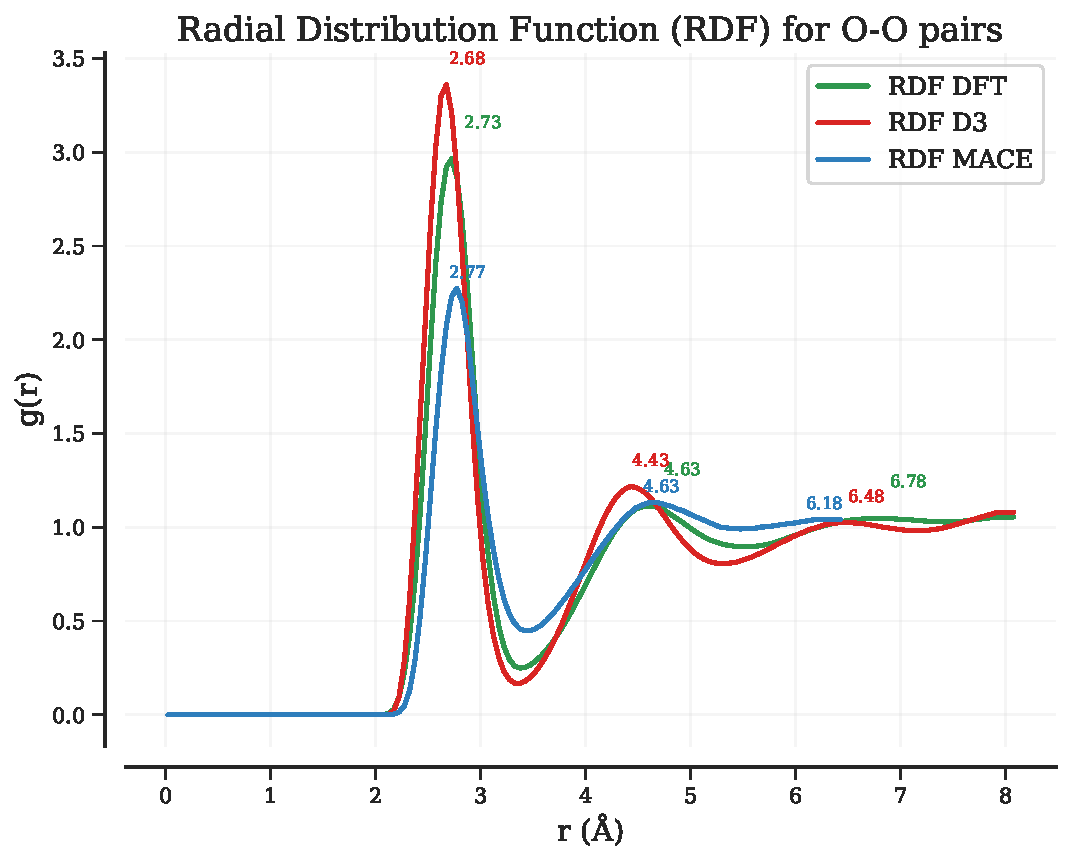
\includegraphics[width=.7\linewidth]{images/rdf_o_o.pdf}
    \caption{Radial distribution function of three models compared for the \(\text{O-O}\) bonds.}
    \label{fig:oh}
\end{figure}


\begin{table}[htbp]
    \centering
    \caption{Comparison of structural parameters across different models.}
    \label{tab:comparison}
    \begin{tabular}{l c c c c}
        \toprule
        \textbf{Method} & \boldmath{$C_N$} & \textbf{Peak $r$ (\AA)} & \boldmath{$r_1$ (\AA)} & \boldmath{$r_2$ (\AA)} \\
        \midrule
        DFT & $\approx 2.26$ & 3.33 & 2.73 & 4.63 \\
        D3 & $\approx 2.31$ & 3.33 & 2.68 & 4.43 \\
        MACE & $\approx 2.04$ & 3.48 & 2.77 & 4.63 \\
        Experiment & 1.8--2.2 & -- & $\approx 2.7$ & $\approx 4.5$ \\
        \bottomrule
    \end{tabular}
    \label{tab:rdf}
\end{table}


The results of the current discussion are summarized in \cref{tab:rdf}
The RDFs of the \(\text{O-O}\) bonds show a more promising seperation between the models. While the dispersion corrected model seems to structure the system most, the MACE model clearly simulates the softest system structuring. In general, every model seems to simulate the bond distances \(r_1\) and \(r_2\) in a good agreement with the experimental values of \(r_{1} \approx 2.7\) \AA, \(r_{2} \approx 4.5\) \AA.
With experimental values for the first coordination number \(C_N\) between \(1.8\) and \(2.2\) only the MACE model seems to replicate the correct coordination number.


